

\tikzset{every picture/.style={line width=0.75pt}} %set default line width to 0.75pt        

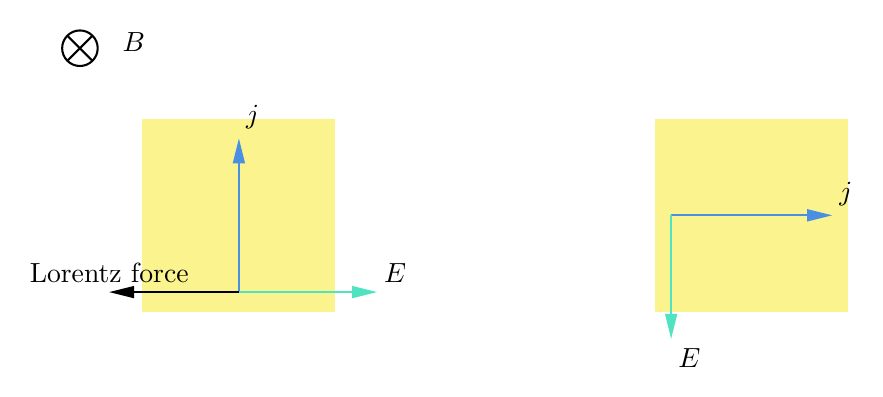
\begin{tikzpicture}[x=0.75pt,y=0.75pt,yscale=-1,xscale=1]
%uncomment if require: \path (0,300); %set diagram left start at 0, and has height of 300

%Shape: Square [id:dp7594515374681072] 
\draw  [draw opacity=0][fill={rgb, 255:red, 248; green, 231; blue, 28 }  ,fill opacity=0.5 ] (100,121) -- (193,121) -- (193,214) -- (100,214) -- cycle ;
%Shape: Square [id:dp3427181984144141] 
\draw  [draw opacity=0][fill={rgb, 255:red, 248; green, 231; blue, 28 }  ,fill opacity=0.5 ] (347,121) -- (440,121) -- (440,214) -- (347,214) -- cycle ;
\draw   (63.84,80.95) .. controls (67.18,77.6) and (72.6,77.6) .. (75.95,80.95) .. controls (79.29,84.29) and (79.29,89.71) .. (75.95,93.05) .. controls (72.6,96.4) and (67.18,96.4) .. (63.84,93.05) .. controls (60.5,89.71) and (60.5,84.29) .. (63.84,80.95) -- cycle ; \draw   (63.84,80.95) -- (75.95,93.05) ; \draw   (75.95,80.95) -- (63.84,93.05) ;
%Straight Lines [id:da9866503409418597] 
\draw [color={rgb, 255:red, 74; green, 144; blue, 226 }  ,draw opacity=1 ]   (146.5,204.5) -- (146.5,132.5) ;
\draw [shift={(146.5,130.5)}, rotate = 90] [fill={rgb, 255:red, 74; green, 144; blue, 226 }  ,fill opacity=1 ][line width=0.08]  [draw opacity=0] (12,-3) -- (0,0) -- (12,3) -- cycle    ;
%Straight Lines [id:da13595332114098047] 
\draw    (146.5,204.5) -- (86,204.5) ;
\draw [shift={(84,204.5)}, rotate = 360] [fill={rgb, 255:red, 0; green, 0; blue, 0 }  ][line width=0.08]  [draw opacity=0] (12,-3) -- (0,0) -- (12,3) -- cycle    ;
%Straight Lines [id:da5681213668237113] 
\draw [color={rgb, 255:red, 80; green, 227; blue, 194 }  ,draw opacity=1 ]   (146.5,204.5) -- (211,204.5) ;
\draw [shift={(213,204.5)}, rotate = 180] [fill={rgb, 255:red, 80; green, 227; blue, 194 }  ,fill opacity=1 ][line width=0.08]  [draw opacity=0] (12,-3) -- (0,0) -- (12,3) -- cycle    ;
%Straight Lines [id:da9071388501116191] 
\draw [color={rgb, 255:red, 74; green, 144; blue, 226 }  ,draw opacity=1 ]   (354.75,167.5) -- (430.25,167.5) ;
\draw [shift={(432.25,167.5)}, rotate = 180] [fill={rgb, 255:red, 74; green, 144; blue, 226 }  ,fill opacity=1 ][line width=0.08]  [draw opacity=0] (12,-3) -- (0,0) -- (12,3) -- cycle    ;
%Straight Lines [id:da36070135647852175] 
\draw [color={rgb, 255:red, 80; green, 227; blue, 194 }  ,draw opacity=1 ]   (354.75,167.5) -- (354.75,225) ;
\draw [shift={(354.75,227)}, rotate = 270] [fill={rgb, 255:red, 80; green, 227; blue, 194 }  ,fill opacity=1 ][line width=0.08]  [draw opacity=0] (12,-3) -- (0,0) -- (12,3) -- cycle    ;

% Text Node
\draw (89,78) node [anchor=north west][inner sep=0.75pt]    {$\boldsymbol{B}$};
% Text Node
\draw (148.5,127.5) node [anchor=south west] [inner sep=0.75pt]    {$\boldsymbol{j}$};
% Text Node
\draw (84,201.5) node [anchor=south] [inner sep=0.75pt]   [align=left] {Lorentz force};
% Text Node
\draw (215,201.5) node [anchor=south west] [inner sep=0.75pt]    {$\boldsymbol{E}$};
% Text Node
\draw (434.25,164.5) node [anchor=south west] [inner sep=0.75pt]    {$\boldsymbol{j}$};
% Text Node
\draw (356.75,230) node [anchor=north west][inner sep=0.75pt]    {$\boldsymbol{E}$};


\end{tikzpicture}
